%%
%% CISC 468 Final Report -- Secure P2P File Sharing Application
%%
\RequirePackage[bookmarksnumbered,unicode]{hyperref}
\documentclass[sigconf,nonacm]{acmart}

\AtBeginDocument{%
  \providecommand\BibTeX{{%
    \normalfont B\kern-0.5em{\scshape i\kern-0.25em b}\kern-0.8em\TeX}}}

\usepackage{tikz}
\usetikzlibrary{arrows.meta,positioning}

\begin{document}

\title{Secure Peer-to-Peer File Sharing with Cross-Language Interoperability}

\author{Selena Zou (20282915, 20sz88@queensu.ca)}
\author{Ayman Zaher (20270677, 20az27@queensu.ca)}

\begin{abstract}
We present a peer-to-peer secure file sharing application consisting of two interoperable clients implemented in Python and C\#.
The application provides mutual authentication via RSA-2048 signatures, confidentiality and integrity via AES-256-GCM, and perfect forward secrecy via ephemeral X25519 key exchange.
Peers discover each other on a local network using multicast DNS and communicate over a custom binary protocol.
Files are encrypted at rest using AES-256-CBC with a password-derived key, and file integrity is cryptographically verified even when obtained through intermediary peers.
The source code is available at \url{https://github.com/azaher1126/Secure_P2P_Files}.
\end{abstract}

\maketitle

\section{Introduction}

Secure file sharing between peers on a local network requires careful coordination of several cryptographic mechanisms: authenticated key exchange, transport encryption, integrity verification, and secure storage.
This project implements a peer-to-peer file sharing system in which two clients, written in Python and C\#, interoperate despite using different cryptographic libraries.

The system follows a layered architecture.
At the lowest layer, peers discover each other via multicast DNS (mDNS), advertising a shared service type on the local network.
Upon connection, peers perform a mutually authenticated handshake in which each peer signs an ephemeral X25519 public key with its long-term RSA-2048 identity key~\cite{paar2024, alaca2026}.
The resulting shared secret is expanded via HKDF into an AES-256-GCM session key used for all subsequent communication.
Above the transport layer, a custom binary protocol supports file list queries, file transfer requests with explicit consent, and key migration notifications.

The Python client uses the \emph{cryptography} library~\cite{pyca} and \emph{zeroconf}~\cite{zeroconf} for mDNS.
The C\# client uses .NET's built-in cryptography namespace supplemented by BouncyCastle~\cite{bouncycastle} for X25519, and Theodicean.Makaretu.Dns.Multicast~\cite{Theodicean} for mDNS.
Both clients implement an identical wire protocol with the same cryptographic algorithms and parameters, enabling seamless cross-language communication.

The remainder of this report is organized as follows.
Section~\ref{sec:requirements} describes how each project requirement is satisfied.
Section~\ref{sec:evaluation} discusses evaluation methodology and known limitations.
Section~\ref{sec:conclusion} presents lessons learned and possible improvements.


\section{Requirements and Implementation}
\label{sec:requirements}

This section describes how each of the eleven project requirements is met.
Table~\ref{tab:crypto} summarizes the cryptographic algorithms and parameters used by both clients.

\begin{table}
  \caption{Cryptographic Algorithms and Parameters}
  \label{tab:crypto}
  \begin{tabular}{p{2.1cm}p{5.5cm}}
    \toprule
    Purpose & Algorithm / Parameters \\
    \midrule
    Identity keys & RSA-2048, PSS padding, SHA-256, MGF1 \\
    Key exchange & X25519 (ephemeral per session) \\
    Key derivation & HKDF-SHA256, salt \texttt{"CISC468-SALT"}, info \texttt{"SessionKey"}, 32-byte output \\
    Transport enc. & AES-256-GCM, 12-byte nonce, 128-bit tag \\
    Storage enc. & AES-256-CBC, PKCS7, random 16-byte IV \\
    Key file enc. & PBKDF2-SHA256, 600{,}000 iterations \\
    File integrity & SHA-256 hash + RSA-PSS signature \\
    Peer fingerprint & First 8 bytes of SHA-256(public key DER) \\
    \bottomrule
  \end{tabular}
\end{table}

\subsection{Peer Discovery}

Peers advertise and discover each other on the local network using mDNS with the service type \texttt{\_securep2p\-files.\_tcp.local.}.
The Python client uses the \texttt{zeroconf} library~\cite{zeroconf} with a \texttt{Service\-Browser} that detects peer arrivals and departures.
The C\# client uses Theodicean.Makaretu.Dns.Multicast~\cite{Theodicean} to advertise a DNS-SD service profile keyed by the peer's fingerprint, filtering out loopback and tunnel interfaces.
Both clients extract the peer's IP address and port from the mDNS response to establish TCP connections.

\subsection{Mutual Authentication}

Each peer possesses a long-term RSA-2048 identity key pair generated at first launch.
During the handshake, the initiator sends its RSA public key in DER format, an ephemeral X25519 public key, and an RSA-PSS signature over the X25519 key.
The responder verifies this signature against the received RSA public key, then replies with its own keys and signature.
Both peers thus prove possession of their respective RSA private keys, achieving mutual authentication.
Figure~\ref{fig:handshake} illustrates this process.

\begin{figure}[h]
  \centering
  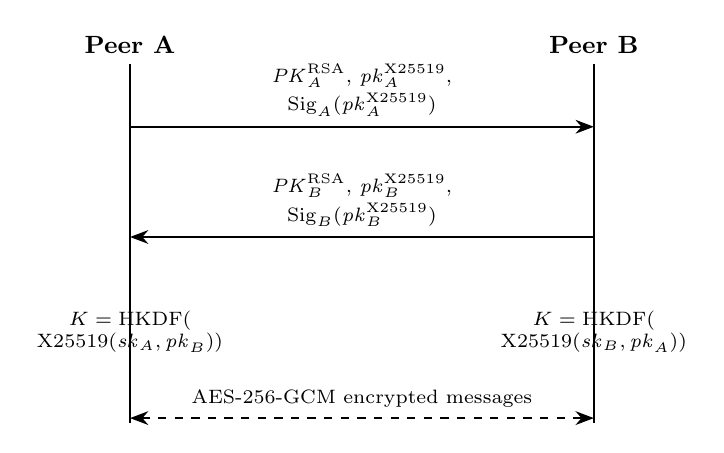
\begin{tikzpicture}[>=Stealth, node distance=4.5cm, font=\small]
    \node (A) {\textbf{Peer A}};
    \node (B) [right=of A] {\textbf{Peer B}};
    \draw[thick] (A) -- ++(0,-4.8);
    \draw[thick] (B) -- ++(0,-4.8);

    \draw[->,thick] ([yshift=-0.8cm]A.south) -- ([yshift=-0.8cm]B.south)
      node[midway,above,align=center,font=\scriptsize] {$\mathit{PK}_A^{\mathrm{RSA}}$, $\mathit{pk}_A^{\mathrm{X25519}}$,\\[1pt] $\mathrm{Sig}_{A}(\mathit{pk}_A^{\mathrm{X25519}})$};

    \draw[<-,thick] ([yshift=-2.2cm]A.south) -- ([yshift=-2.2cm]B.south)
      node[midway,above,align=center,font=\scriptsize] {$\mathit{PK}_B^{\mathrm{RSA}}$, $\mathit{pk}_B^{\mathrm{X25519}}$,\\[1pt] $\mathrm{Sig}_{B}(\mathit{pk}_B^{\mathrm{X25519}})$};

    \node[font=\scriptsize,align=center] at ([yshift=-3.4cm]A.south) {$K = \mathrm{HKDF}($\\$\mathrm{X25519}(\mathit{sk}_A, \mathit{pk}_B))$};
    \node[font=\scriptsize,align=center] at ([yshift=-3.4cm]B.south) {$K = \mathrm{HKDF}($\\$\mathrm{X25519}(\mathit{sk}_B, \mathit{pk}_A))$};

    \draw[<->,thick,dashed] ([yshift=-4.5cm]A.south) -- ([yshift=-4.5cm]B.south)
      node[midway,above,font=\scriptsize] {AES-256-GCM encrypted messages};
  \end{tikzpicture}
  \caption{Mutually authenticated handshake protocol. Each peer signs its ephemeral X25519 public key with its long-term RSA-2048 private key. Both peers derive the same session key $K$ via X25519 key agreement and HKDF.}
  \Description{Sequence diagram showing the two-message handshake between Peer A and Peer B, followed by symmetric encrypted communication.}
  \label{fig:handshake}
\end{figure}

\subsection{File Requests and Consent}

Peers can request to download a file (\texttt{ReqToReceive}) or offer to upload a file (\texttt{ReqToSend}).
The receiving peer is prompted for consent and replies with a \texttt{ConsentResponse} message indicating acceptance or denial.
File data is transmitted only after the recipient explicitly accepts, ensuring that no file transfer occurs without user consent.

\subsection{File List Queries}

A peer may request another peer's list of shared files at any time without requiring consent.
The response includes each file's name, SHA-256 hash, owner fingerprint, and an RSA-PSS signature over the concatenation of the filename and hash.
This metadata enables integrity verification even when the file is later obtained from a different peer.

\subsection{Indirect File Transfer and Integrity}

When peer~B requests a file originally shared by an offline peer~A from an intermediary peer~C, the system preserves peer~A's original RSA-PSS signature and owner fingerprint in the file metadata.
Peer~B retrieves peer~A's public key from its contact store, recomputes the SHA-256 hash of the received file, and verifies the signature against the original owner's key.
A verification failure indicates tampering, and the file is rejected.
This ensures file integrity regardless of the transfer path.

\subsection{Key Migration}

If a peer's long-term RSA key is compromised, the peer generates a fresh RSA-2048 key pair and broadcasts a \texttt{KeyMigration} message to all active sessions.
This message contains the new public key, a 16-byte random replay nonce, and an RSA-PSS signature computed over the concatenation of the new key and nonce using the \emph{old} private key.
Each recipient verifies the signature with the sender's currently trusted public key, checks the nonce against a set of previously seen nonces to prevent replay attacks, and updates its contact store upon successful verification.
All existing sessions are terminated, forcing re-authentication with the new key.

\subsection{Confidentiality and Integrity}

All post-handshake communication is encrypted with AES-256-GCM~\cite{paar2024}, which provides both confidentiality and integrity in a single authenticated encryption operation.
Each message uses a fresh 12-byte random nonce and produces a 128-bit authentication tag.
The wire format prepends a one-byte message type and a four-byte payload length to the nonce, ciphertext, and tag, as shown in Table~\ref{tab:wireformat}.

\begin{table}
  \caption{Post-Handshake Wire Format}
  \label{tab:wireformat}
  \begin{tabular}{ccp{3.5cm}}
    \toprule
    Offset & Size & Field \\
    \midrule
    0 & 1\,B & Message type \\
    1 & 4\,B & Ciphertext length (big-endian) \\
    5 & 12\,B & GCM nonce \\
    17 & var. & Ciphertext \\
    --- & 16\,B & GCM authentication tag \\
    \bottomrule
  \end{tabular}
\end{table}

\subsection{Perfect Forward Secrecy}

Each session uses a freshly generated ephemeral X25519 key pair.
The session key is derived from the ephemeral shared secret via HKDF-SHA256, and the shared secret is zeroed from memory immediately after derivation.
Long-term RSA keys are used only to authenticate the ephemeral keys and play no role in session key derivation.
Consequently, compromise of a long-term RSA private key does not allow an attacker to decrypt any past session.
The C\# client further enforces a five-minute session timeout, after which a new handshake is required.

\subsection{Secure Local Storage}

Files stored on disk are encrypted with AES-256-CBC using PKCS7 padding.
A 32-byte master key is derived from the user's password via PBKDF2-SHA256~\cite{vanoorschot2021} with 600{,}000 iterations and a random 16-byte salt stored separately.
Each encrypted file is prefixed with a random 16-byte initialization vector.
The RSA private key is similarly encrypted with the master key.
An attacker who obtains the device must perform an expensive brute-force attack against the password-derived key to access any stored data.

\subsection{Error Handling}

Both clients display informative messages for all error conditions.
Handshake signature verification failures result in a connection refusal with a clear warning.
Tampered files are rejected with a message indicating that integrity verification failed.
Network errors, consent denials, and unavailable peers all produce user-facing messages describing the issue.

\subsection{Test Cases}

Both clients include test suites that verify correctness under normal and adversarial conditions.
The Python client contains module-level tests for AES-CBC and AES-GCM round-trips, RSA-PSS signature generation and verification, handshake key agreement, message serialization and deserialization for all protocol message types, mDNS peer discovery, and file encryption round-trips.
The C\# client uses xUnit~v3 with dedicated test classes for message framing (including tampered-ciphertext detection and session expiry), all message types, key migration signature verification and replay rejection, file signature verification with hash mismatch detection, fingerprint computation, and user configuration consistency.


\section{Evaluation and Limitations}
\label{sec:evaluation}

We evaluated the application by running both clients on the same local network and verifying all functional and security requirements.
The test suites confirm correct cryptographic operations: encryption round-trips produce identical plaintext, signature verification rejects modified data, and tampered ciphertexts raise authentication errors.
Cross-language interoperability was validated by performing handshakes, file list queries, file transfers, and key migrations between the Python and C\# clients.

Several limitations remain.
First, the HKDF salt is a fixed string (\texttt{"CISC468-SALT"}) rather than a random value exchanged during the handshake; a per-session random salt would provide stronger key separation.
Second, the system uses a trust-on-first-use model for identity keys: there is no certificate authority or out-of-band verification mechanism, so the first connection to a peer must be assumed trustworthy.
Third, mDNS-based peer discovery operates only on local networks; extending the system to the Internet would require a protocol such as a distributed hash table.
Fourth, file transfers are not chunked, so very large files must fit entirely in memory during transmission.
Fifth, the key migration replay nonce set is maintained in memory and is not persisted across application restarts, which could allow a replay attack if the application is restarted before processing a replayed migration message.


\section{Conclusion}
\label{sec:conclusion}

This project demonstrates that two independently implemented clients can securely interoperate using a shared cryptographic protocol.
The primary lesson learned is that cross-language interoperability requires precise agreement on serialization formats, byte orderings, and algorithm parameters; even minor discrepancies in padding or key encoding prevent successful communication.
We also observed that designing for perfect forward secrecy with ephemeral key exchange adds minimal complexity when using modern libraries that support X25519 and HKDF natively.

Possible improvements include replacing the fixed HKDF salt with a per-session random value, adding out-of-band key verification (e.g., safety number comparison as in the Signal protocol), implementing chunked file transfers for large files, persisting replay nonce state to disk, and extending peer discovery beyond the local network using a distributed hash table.


\bibliographystyle{ACM-Reference-Format}
\bibliography{references}

\end{document}
